%
% Draft  document birthcoat.tex
% Questions regarding control of fibre diameter and length growth rate
%
 
\documentclass[titlepage]{article}  % Latex2e
\usepackage{graphicx,lscape,subfigure}
\usepackage{bm}
\usepackage{textcomp}
\usepackage{tikz}
 

\title{Questions regarding role of some birthcoat characteristics in evolution of domesticated sheep breeds and in fleece improvement}
\author{Neville Jackson, Philip  Moore, Paul Swan, and Jim Watts}
\date{26 Nov 2018} 

 
\begin{document} 
 
\maketitle      
\tableofcontents

\clearpage
\section{Introduction} 
This is a  very narrow review of the significance of sheep birthcoats. What we are trying to do is  develop ideas as to how any why birthcoat characteristics are important,  firstly to the lamb, and secondly to the breeding of wool sheep, particularly  in relation to genetic control of fibre diameter, and the evolutionary development of domesticated sheep.


\section{What is a birthcoat?}
Lambs are born with at least some of their follicles already growing a wool fibre. The term {\em birthcoat} refers to those fibres which have grown from the follicle in-utero and which therefor protrude from the skin at birth, forming a protective coat for the lamb. There are various types of fibre in a lamb fleece, recognizable by the shape of the fibre tip and the presence of medullation. There is a good summary in Onions(1962)~\cite{onio:62} and we are going to save repetitive effort by reproducing material form Onion's book here.

First, we have a description of fibre types (Figure~\ref{fig:fibretypes})
%\documentclass{article}
%\usepackage{graphicx,subfigure}
%\begin{document}

\begin{figure}[!h]
  \centering
   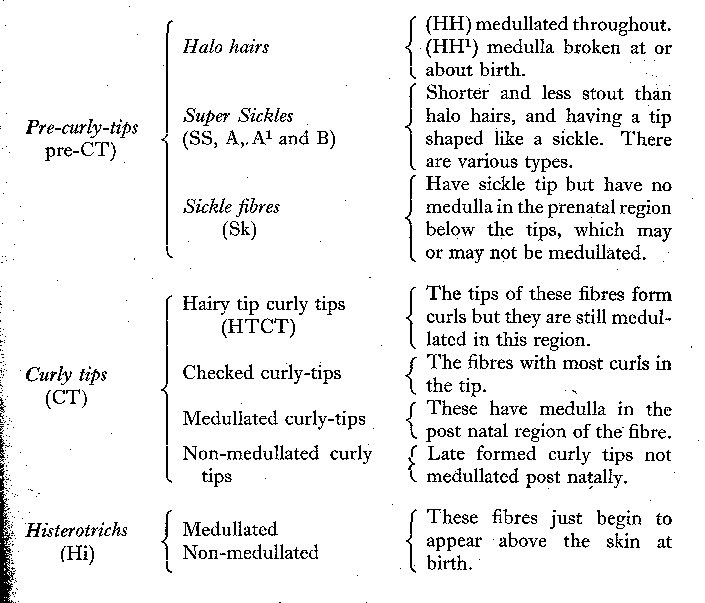
\includegraphics[width=1.0\textwidth]{fibretypes2.png}
  \caption{Text extract from Onions(1962)~\cite{onio:62} defining birthcoat fibre types}
  \label{fig:fibretypes}
\end{figure}

%\end{document}


These descriptions come from Dry(1934)~\cite{dryf:34}. The three main types of fibre are distinguished by their length and the crimp shape and degree of medullation of their tips.

Figure~\ref{fig:onions} illustrates these fibre types, which are aligned so that the position of the skin level at birth is on a common horizontal line.
%\documentclass{article}
%\usepackage{graphicx,subfigure}
%\begin{document}

\begin{figure}[!h]
  \centering
   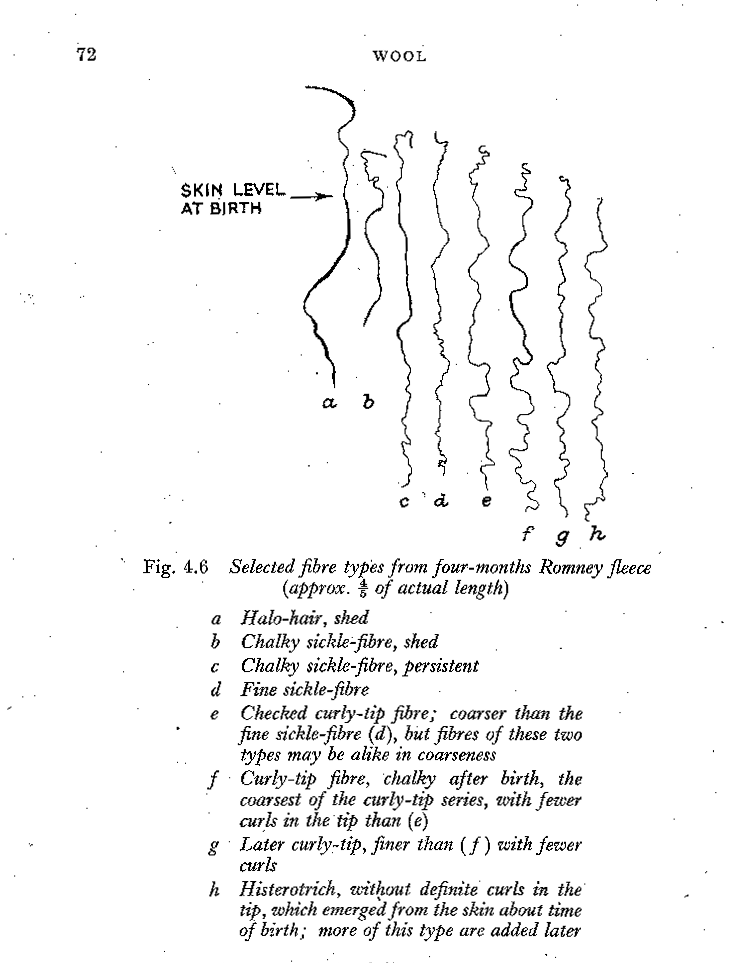
\includegraphics[width=1.0\textwidth]{onions2.png}
  \caption{Figure from Onions(1962)~\cite{onio:62} showing fibre types from a Romney lamb with the  fibres aligned according to the position of the skin level at birth}
  \label{fig:onions}
\end{figure}

%\end{document}


It is a convention, in studying lamb fibre types, to harvest fibres when lambs are about 1-2 months old, so that all fibre types including {\em histerotrichs} are present, and the process of breaking off of the birth tips has not yet commenced. So the fibres drawn in Figure~\ref{fig:onions} are strictly more than just the birthcoat, they are {\em lamb fibre types} and Dry(1934)~\cite{dryf:34} refers to them as such.

The thickened regions of these hand drawn fibre representations are meant to indicate presence of medullation. The region immediately above the skin level at birth is known as the {\em pre-natal check}. It apperars only on the per-CT and CT fibre types, not on the histerotrichs.

Figure~\ref{fig:follicletypes} which is also reproduced from Onions, but which is  actally  a modified version of a Table from Carter(1955)~\cite{cart:55}, shows the postulated correspondence of follicle types and their initiation timings with Dry's fibre types.
%\documentclass{article}
%\usepackage{graphicx,subfigure}
%\begin{document}

\begin{figure}[!h]
  \centering
   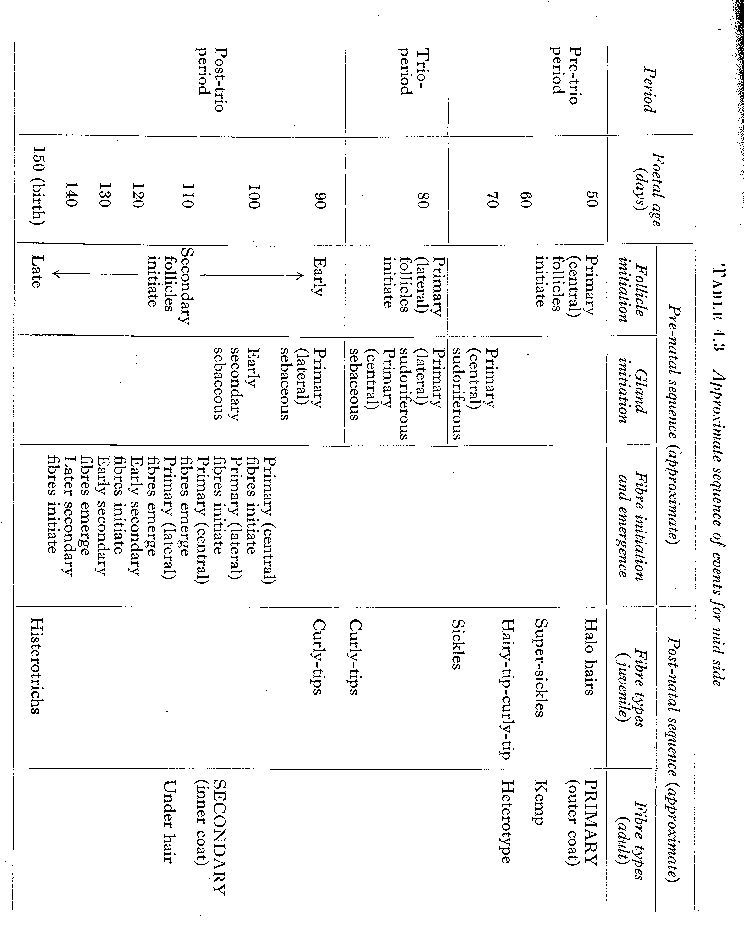
\includegraphics[width=1.0\textwidth]{follicletypes2.png}
  \caption{Table from Onions(1962)~\cite{onio:62} setting out proposed relationships between fibre types and follicle types (after Carter(1955)~\cite{cart:55})}
  \label{fig:follicletypes}
\end{figure}

%\end{document}


Basically Primary central follicles make sickle tips, Primary lateral follicles make curly tips, and Secondary follicles make histerotrichs. So all the fibres which have a portion above skin level at birth have come from primary follicles, and only these fibres show a pre-natal check.

Much of the appeal of {\em lamb fibre types} is that they offer a means of identifying fibres which have grown from primary central, primary lateral, and secondary folicles. They do not offer a means of distinguishing fibres from secondary orignal follicles from fibres from secondary derived follicles. 

\section{Prenatal check}
Just before birth, the follicles which are already growing fibres change the fibre growth suddenly, altering the length growth rate, the fibre diameter, and the fibre crimp or curvature. There is a tiny region of very fine fibre diameter, and then the fibre assumes its {\em post-check} growth behaviour, which is not usually the same as the growth which occurred {\em pre-check} in the foetus.

The tiny thinned prenatal check region is responsible for the birthcoat tips of a lambs fleece breaking off. The tips of fibres are gone by about 3 monthes, unless the fleece is coated to retain them.  The phenomenon is most obvious in the Suffolk breed,  where the pre-check tips are pigmented but the post-check fibres are not, so the fleece changes from black to white as the fibre tips break off. Sometimes this phenomenon is referred to as {\em birthcoat shedding}. It is not shedding in the sense of the follicles shutting down and forming a {\em brush end}, it is simply a mechanical break, similar to a tenderness break. 

The fibres with the most prominant change between pre-check and post-check regions are referred to as being {\em checked}. Actually all fibres present at the time of check are checked to various degrees, and it is likely that all follicles are checked, even those not growing a fibre at birth.  Check may  be a systemic phenomenon, although its timing and extent varies over the body of the sheep, and we have cause ( see later) to think that it is of local causal origin.

There is a lot about the prenatal check phenomenon that remains unexplained. We commence with a statement from Dry(1965)~\cite{dry:65}

\begin{quote}
 "The indeterminate growth of most fibres of domesticated sheep is a trichological oddity which has long been attributed to the prenatal check"
\end{quote}

You can read the whole of Dry(1965)~\cite{dry:65} and find not a shred of evidence  supporting this statement, until, right at the end we find the claim repeated

\begin{quote}
" Something unusual happens well before birth, believed to cause that enduring anmoly, indeterminate growth, ...."
\end{quote}

So Dry is either stating something which obvious or common knowledge, or he is making an intuitive claim, without explanation.

We have to ask "How could a prenatal check cause follicles to go permanently into the Anagen phase of the hair growth cycle?" . If prenatal check is really the magic trigger which sends domesticated sheep into continuous growth, we had better understand {\em how} it works.

So, does anyone else think the same as Dry?  There is a review  by Burns(1983)~\cite{burn:83} which makes a lot of summary statements, again without presenting the evidence. Here are some examples
\begin{quote}
" Under the influence of domestication the coat of the sheep has been changed in two opposite directions. In temperate and subtropical environments the outer coat became reduced in coarsness while the undercoat became longer and less fine, and moulting was reduced or totally lost. These changes were associated with, and possibly caused by, something that happend to primary follicles at about 100 to 120 days of foetal age. At this time, in fine wooled breeds, the bulbs of these follicles have actually been seen to be reduced in size, and measurements of fbre growth show that it is delayed at this period. In coarse wooled sheep the effect is not so obvious, but that it does occur is shown by the shape of the tips of fibres in the birthcoat of lambs"
\end{quote}
and 
\begin{quote}
"Dry considered that even wild sheep show some signs of the prenatal fibre check, but that it has been much intensified in fleece bearing breeds, and is responsible for the loss of moult, and, according to its intensity, affects the fineness and medullation of the wool. He considered, however, that there are differences in the wool growth potential of different sheep ( which he called differences in {\em base}), so that there is a complex interaction between base and check"
\end{quote}

 from Burns we can confirm the following
\begin{itemize}
\item Dry really did think that prenatal check caused indeterminate growth. Burns will only concede that it is associated with loss of moult and may be a cause.
\item Follicle bulbs reduce in size at the prenatal check. 
\item All breeds, even wild sheep, have a prenatal check, but it varies in intensity
\item Dry introduced another concept called {\em base}  which seems to be something like 'what the fibre would have been if it was not checked'. We might speculate that {\em base }  is equivalent to the number of papilla cells in the follicle bulb. More on this later.
\end{itemize} 

 Burns makes another important observation
\begin{quote}
"Dr Dry noticed that regularly in Wensleydales, and occasionally in other breeds, the fibre type array commenced with sickle fibres or early curly tips which were finer than the fibres which followed them. He picturesquely calle these arrays "beheaded" or "truncated". The full significance of these arrays was not realised until many years after he named them"
\end{quote}
Nowhere does Burns say what this "full significance" is.  We think we know . That is the type of birthcoat produced by SRS Merino sheep. It means that they have a fine {\em base} or, in our modern terminology, not many papilla cells in primary follicles. 

So the size  (ie diameter) of the sickle tips is a measure of {\em base} and of number of papilla cells in primary follicles.  Why? Because primary follicles ( especially primary central follicles) develop without a {\em locale}, that is without any close surrounding follicles. So the fibre diameter is only determined by papilla cell number. In all other follicles, and in primary follicles after the check, diameter is determined by both papilla cell number and {\em locale}.

For a full discussion of the causes of fibre diameter in individual follicles and evidence for the {\em locale} effect, see the Jackson, Swan and Watts(2018)~\cite{jackswan:18} document.

There is data on fibre length growth rates in utero in the thesis of Side(1964)~\cite{side:64}. Side determined fibre length growth rates using autoradiographic techniques. His graphs of the length growth rates of the various fibre types show the following
\begin{itemize}
\item a check in growth rate of all fibres at around 120 days - this is Dry's prenatal check
\item in some sheep a second check at around 135-140 days, in other words, immediately before birth
\item all fibres change growth in unison
\item the coarsest and earliest formed fibres have the highest growth rate
\item the severity of check varies with breed of sheep and with body site.
\end{itemize}
Side did not measure diameters on his autoradiographs.

In a chapter by Side and Rudall(1964) in a dermatology book the following comment appears.
\begin{quote}
"It is our first prenatal check which corresponds to the main features of the prenatal check in Dry's sense, which his extensive work over the last 35 years suggests to be associated with the relatively persistent growth of the fleece. The term has descriptive value for the visible morphology of birthcoat fibres and for their growth-rate curves, but its physiological interpretation remains problematical"
\end{quote}
and also the following

\begin{quote}
"Theories to acount for the prenatal check have been produced, and fall into two main classes. One attributes it to a systemic, probably endocrine, change occuring at the relevant phase of gestation. The other seeks its cause in local interactions between follicles (Galpin, 1935); in its most recent form, this theory specifically suggests that the depression of growth in some primary fibres is caused by competition for substrate from neighbouring follicles when these start to produce fibres (Fraser, 1951, 1952, 1953)."
\end{quote}
 
So modern work favours local over  systemic effects, as an explanation of prenatal check.  We come back to that later. People keep referring to Dry's idea of persistent growth evolution being linked to prenatal check, but there is still no data and no explanation of how a check might trigger persistent growth. 

Side(1964)~\cite{side:64} concludes his thesis with the following
\begin{itemize}
\item evidence suggests that neither of the two prenatal checks is of systemic origin
\item onset of the first ( ie Dry's) prenatal check coincides with the onset of secondary fibre production
\item \begin{quote}
"It is suggested that the primitive prenatal check is an adaptation whereby a complete infant pelage is produced by follicles which grow only the outer coat of the adult, and that it has been accentuated in the evolution of the fleece by progressive extension of secondary fibre initiation into prenatal life."
\end{quote}
\item \begin{quote}
"The relationship between the (accentuated) prenatal check of domestic sheep and the evolution of relatively persistent growth of the fleece remains problematical."
\end{quote}
\item \begin{quote}
"...presence of a primitive prenatal check in wild species, evolved as an adaptation for early independence in a rigorous environment, was a prerequisite for the subsequent evolution of the fleece under human influence, making possible (but not inevitable) the transformation of kemp to wool by selection for more, larger, and earlier developing secondary fibres."
\end{quote}
\end{itemize}

Given that Side actually has some data to back up his statements, I think we have to concur with his conclusions.  The original prenatal check in primitive sheep is an adaptation allowing the newborn lamb to have a two-coated fleece, and the accentuated prenatal check in domestic species is simply a byproduct of selection for a fleece of uniform fibre diameter. Continuous growth may also be a byproduct of domestic selection for a uniform fleece. Prenatal check is a correlated side effect, not a cause of continuous growth.


\section{Our birthcoat hypothesis}
We can sum it up in one sentence

{\em The processes which control fibre diameter and length growth rate and fibre curvature in the foetus are the same as those which control them in the adult fleece}

The only additional thing to note is that some of the external ( to the follicle) factors influencing these processes are more extreme and more varying in the foetus.

Our interpretation of the descriptive work of earlier workers is that "base" is papilla cell number, and "check" is a locale effect. In some of Dry's references to "base" it is clear he is referring to total papilla cell number, in other cases he means papilla cell number per follicle.  Base is woolgrowing potential, either per follicle or per animal. There is no doubt that papilla cell number is woolgrowing potential - it regulates the ability of the follicle bulb to produce cortical cells.

So what is this {\em locale} effect? You have to look at Jackson, Swan and Watts(2018) for detail, and evidence.  It is simply the environment surrounding each follicle, including the number and size and activity of surrounding follicles. The clearest demonstration of locale effect is the sickle tip on primary central fibres. That is the closest thing you will ever get to the output of a follicle in the absence of any locale effect. What do you get? - large fibre diameter, fast length growth rate, and the fibre growing in a continuous curve ( like a coiled up hose). All later fibre growth is finer, shorter, and forms a wave-like crimp. The surrounding follicles depress the woolgrowing potential of the follicle and the interaction with surrounding fibres changes the continuous curve into a crimp. You can see the effect even in utero - the curly tips are finer than the sickle tip and are crimped. There is one point at which the locale is very depressive, and this is the prenatal check point. It coincides in time with the massive development of secondary follicles. In the post-birth period, the locale effect can reduce, or can remain strong - which of these probably depends on development of secondary derived follicles.

\section{Birthcoats and evolution}
What role have birthcoats played in the evolution of domestic sheep, and in particular development of the Merino?

We think it would be fair to assume that man has never applied artificial selection directly for birthcoat characteristics. On the other hand, natural selection will always favour the type of birthcoat which provides the lamb with a protective two-coated fleece.  Lambs of wild sheep are two coated, with coarse long fibres from primary central follicles , and fine shorter fibres from primary lateral follicles.

The question is, to what extent has man's artificial selection for a uniform adult fleece modified the lamb birthcoat? The answer is that a number of things have happened in line with the main stages of domestic sheep evolution. We summarize this in Table~\ref{tab:evolstages}
%\documentclass{article}
%\usepackage{lscape}
%\begin{document}

\begin{center}
\begin{landscape}
\begin{table}[h]
\caption{Approximate measurements for sheep representing Ryder's 4 stages of Merino evolution, extended to the modern SRS Merino. Sources lines 1 to 3 Ryder(1992)~\cite{ryde:92}, line 4 Carter(1968)~\cite{cart:68}, line 5 Watts(2017)~\cite{watt:17}. Correlated changes in birthcoat are not evidence based, but are inferred from our present understanding of birthcoats. Base is the primary central fibre before prenatal check, Post-check is the primary fibres after prenatal check, ie the 'strength' of the check} 
\label{tab:evolstages}
\vspace{0.1in}
\begin{tabular}{|p{0.6in}|p{0.6in}|p{0.4in}|p{0.4in}|p{0.6in}|p{0.7in}|p{0.7in}|p{0.7in}|p{0.7in}|}  \hline
 
  \multicolumn{2}{|c|}{Evolution} & \multicolumn{5}{c|}{Adult Fleece} & \multicolumn{2}{c|}{Birthcoat Fibres} \\ \hline
  Stage &  Chronology &  Dp & Ds & S/P ratio & Medullation & Shedding  & Base & Post-check \\ \hline
  Wild   & Neolithic (10000-3000BC) & 80-200 & 14-16 & 3-5 & Outercoat kemp & Undercoat sheds & Coarse sickle tip & Very Coarse fibre \\ \hline
  Hairy Medium Wool & Bronze Age (3000 - 1000BC) & 40-140 & 18-28 & 4-5 & Outercoat hair & Undercoat sheds & Coarse sickle tip & Medium fibre \\ \hline
  Generalised Medium Wool & Iron Age (1000BC - 700 AD) & 20-50 & 18-35 & 5-7  & No outercoat? & Secondaries continuous & Coarse sickle tip & Fine fibre \\  \hline
  Finewool Merino & (1200AD - present) & 18-20 & 17-19 & 15-25 & No outercoat & Secondaries continuous & Medium sickle tip & Fine fibre\\  \hline
  SRS Fine Merino & (1990AD - present) & 14-17 & 17-19 & 25-40 & No outercoat & Secondaries continuous  & Fine long sickle tip  & Fine fibres \\ \hline
\end{tabular}
\end{table}
\end{landscape}
\end{center}

%\end{document}

Table~\ref{tab:evolstages} is from Jackson(2017)~\cite{jack:17} (Table 3 in that document) with some birthcoat information appended. What Table~\ref{tab:evolstages} shows is that for all of the stages of evolution up to and including the modern Fine Merino, fine uniform fibres ( particularly primary fibres) have been obtained by successively stronger checking. Not just the severe short-term prenatal check but continued checking of the fibre growth at all stages into adult life. What is surprising is that the development of the SRS Merino has taken a different approach, by starting out primary fibres with a fine "base" ( ie reduced papilla cell number), so that they do not need to be strongly checked to remain fine into adult life. One of the distinguishing features of the SRS Merino is that this different approach has been more successful than the previous 3000 years of breeding for fibre uniformity via successively stronger prenatal checks.

We have noted above that the SRS Merino is not the only sheep breed to have taken the fine "base" approach. The Wensleydale breed - a British longwool breed developed in Yorkshire in the 19th century - also has fine sickle tips in the birthcoat, and its adult fleece has all the characteristics of the SRS Merino except at a lower fibre density and a coarser mean diameter. There are no available Dp and Ds data for the Wensleydale breed, but one would expect a Dp/Ds ratio of 1.0 or less. The domestic evolution of longwools has taken a similar path to the SRS Merino. What British longwools have missed is the huge step toward fine primary fibres and large S/P ratio which distinguishes the Merino from all other breeds.  It has been suggested that Merinos may have acquired this large step from the Rex gene, which has similar effects in rodents and cats.

\section{Birthcoats and fleece improvement}
Some of the points of the previous section are relevant here too, but what we are focussed on here are the various selection methods used for Merino sheep in Australia, and  the effect they might have on the two birthcoat factors "base" and "check". 

We have identified "base" with papilla cell number. We think the diameter of the sickle tip on Pc fibres in the birthcoat would be a useful measure of this. However there are no available measurements of sickle tip diameters. What has tended to have been used is Dp - the diameter of primary fibres in the adult fleece. However this may reflect "check" as well as "base". 

Subjective scores for birthcoat 'hairiness' may be more useful than Dp as an indicator of primary follicle papilla cell number. Birthcoat hairiness score has a high genetic correlation with Dp ( 0.70 +- 0.03) and is not correlated with Ds ( -0.14 +- 0.04).  Because hairy birthcoats are associated with better lamb survival in harsh conditions, there may be natural selection for a large "base" or a large papilla cell number in primary follicles. This may explain why sheep with a coarse adult Dp keep occurring in modern Merino flocks.

Selection for clean wool weight tends to dramatically increase Ds ( genetic correlation 0.63 +- 0.06) but has little effect on Dp (genetic corelation -0.01 +- 0.06).  So clean wool weight selection would be neutral in relation to "base" or papilla cell number in primary follicles. If, however, one adds some culling against coarse fibre diameter, there may be pressure for a large "check" effect on secondary fibres. This "check" would have to come from an increase in density.

The challenge would seem to be to find ways of increasing the total number of papilla cells, but ensuring that they are shared among a large number of follicles, so that the number per follicle is small and the diameter therefore fine. The hypothesis regarding papilla cell dynamics of Moore etal(1984, 1989, 1998)~\cite{moor:84}~\cite{moor:89}~\cite{moor:98} provides one suggested way of doing this - keep Dp fine. Another possibility, arising from present considerations, is to keep the sickle tips of the birthcoat fine. The latter may actually be more effective, as it measures "base" without any "check" effect.

\section{Discussion}
This questioning document arose because we encountered a somewhat surprising statement from Dr Dry that "prenatal-check"  was somehow involved in the evolution of continuous growing fibres in domestic sheep breeds. We have failed to find any justification for a causal relationship, it is just that continuous growth and a stronger prenatal check tend to occur together, probably both as a result of some other factor.

We have , however, unearthed some other useful concepts. We summarise these below
\begin{itemize}
\item we identify Dry's "base" with papilla cell number
\item we identify Dry's "prenatal check" with the {\em locale} effect deveoped in Jackson , Swan and Watts(2018)~\cite{jackswan:18}
\item we propose diameter of Pc fibre sickle tips in the birthcoat as a measure of "base" unaffected by "check"
\item we assert that adult Dp is a useful measure of "base" but can also be affected by "check"
\item  we think that clean wool weight selection is neutral in relation to "base" but can require a strong "check" to counter correlated change in Ds
\item most of the evolution of domestic breeds has been via increase in severity of "check". Only two recent developing breeds target "base"
\item continuous growth remains a mystery
\end{itemize}

This is an ideas document, not a scoientific paper. It doesnt prove anything. Its outcome is a framework for further work.  It has already helped with the diameter control study ( Jackson , Swan and Watts(2018)~\cite{jackswan:18}) and it may provide some clues to unravelling the evolution of domestic sheep, particularly recent evolution of the Merino.

It is review old work and find the concepts have a modern interpretation



\begin{thebibliography}{99}
\bibitem{burn:83}
Burns, M. (1983) The Wensleydale Longwool Sheep. ARK, Monthly Journal of the Rare Breeds Survival Trust. Vol X, Number 2 - Febuary 15, 1983

\bibitem{cart:43}
Carter, H.B. (1943) Studies in the Biology of the Skin and Fleece of Sheep. 1. The development and general histology of the follicle group in the skin of the Merino. 2. The use of the tanned sheepskin in the study of follicle population density. 3. Notes on the arrangement, nomenclature, and variation of skin folds in the Merino. CSIR Bulletin No 164, Melbourne, 1943

\bibitem{cart:47}
Carter, H.B. and Hardy, M.H. (1947) Studies in the Biology of the Skin and Fleece of Sheep. 4. The hair follicle group and its topographical variations in the skin of the Merino foetus. CSIR Bulletin No 215, Melbourne, 1947

\bibitem{cart:55}
Carter, H.B. (1955) The hair follicle group in sheep.  Animal Breeding Abstracts 23:101-116

\bibitem{cart:68}
Carter,H.B. (1968) Comparative Fleece Analysis Data for Domestic Sheep. The Principal Fleece Staple Values of Some Recognised Breeds. Agricultural Research Council, 1968


\bibitem{dryf:34}
Dry, F.W. (1934) New Zealand J. Agric. 49:269-277

\bibitem{dry:65}
Dry, F.W. (1965) Lamb Fibre Types. Biology of the Skin and Hair Growth. ed Lyne, A.G. and Short, B.F. (1965) Angus and Robertson, Sydney, 1965.

\bibitem{dunl:74}
Dunlop, A.A., and McMahone P.R. (1974)  The relative importance of sources of variation in fibre diameter for Australian Merino sheep. Aust. J. agric. Res. 25:167-81

\bibitem{fras:51}
Fraser, A.S. and Short, B.F. (1951) Competition between skin follicles in sheep. Nature 167:202-203

\bibitem{fras:52}
Fraser, A.S. and Short, B.F. (1952) Competition between skin follicles in sheep Aust. J. agric. Res. 3(4):445-452

\bibitem{fras:53}
Fraser, A.S.(1953) Factors in the genetic determination of fleece structure in sheep. J. Genet. 51:222-236

\bibitem{fras:60}
Fraser, A.S. and Short, B.F. (1960) The Biology of the Fleece. Animal Research Laboratories Technical Paper No 3. CSIRO, Australia, 1960

\bibitem{hend:65}
Henderson, A.E., (1965) Relationship of wool follicle and wool fibre dimensions. Biology of Skin and Hair Growth. Proc. Symposium Canberra, Aust, 1964 Ed A.G Lyne and B.F Short.

\bibitem{hori:53}
Horio, M. and Kondo, T. (1953) Text. Res. J. 23:373

\bibitem{jack:16}
Jackson, N. and Watts, J.E. (2016) Staple crimp formation in the fleece of Merino sheep. Unpublished manuscript, 18 May 2016.

\bibitem{jack:17}
Jackson, N. (2017) What are the defining characteristics of primitive sheep relative to a modern Merino sheep? URL https://github.com/nevillejackson/atavistic-sheep/mev-rewrite/supplementary/primitive/primitive.pdf

\bibitem{jack:18}
Jackson, N. and Moore, G.P.M. (2018)
Dynamics of pre-papilla cell numbers in sheep foetus and effect on follicle development URL https://github.com/nevillejackson/Fleece-biology/tree/master/pre-papilla-cells/ppcell.pdf

\bibitem{jackswan:18}
Jackson, N. , Swan, P.G. , and Watts, J.E. (2018) Questions regarding developmental control of fibre diameter and fibre length growth rate in sheep. URL https://github.com/nevillejackson/Fleece-biology/blob/master/diamlen/diamlen.pdf

\bibitem{moor:84}
Moore G.P.M. and Jackson, N. (1984) An hypothesis implicating a founder cell pop
ulation in the regulation of wool follicle formation and distribution in sheep s
kin. J. Embryol. Exp. Morph. 82 (Suppl), 259

\bibitem{moor:89}
Moore G.P.M., Jackson, N., and Lax, J. (1989) Evidence of a unique developmental mechanism specifying both wool follicle density and fibre size in sheep selected for single skin and fleece characters. Genet. Res. Camb. 53:57-62

\bibitem{moor:98}
Moore, G.P.M., Jackson, N., Isaacs, K., and Brown, G (1998) J. Theoretical Biology 191:87-94

\bibitem{nay:66}
Nay T. (1966) Wool follicle arrangement and vascular pattern in the Australian Merino. Aust. J. agric. Res. 17:797-805

\bibitem{nayj:73}
Nay, T. and Jackson, N. (1973) Effect of changes in nutritional level on the depth and curvature of wool follicles in Australian Merino sheep. Aust. J. Agric. Res. 24:439-447

\bibitem{onio:62}
Onions, W.J. (1962) Wool: an introduction to its properties, varieties, uses
     and production. Ernest Benn limited, London, 1962

\bibitem{prie:65}
Priestley, G.C. and Rudall, K.M. (1965) Modifications in the Huxley layer associated with changes in fibre diameter and output. Biology of Skin and Hair Growth. Proc. Symposium Canberra, Aust, 1964 Ed A.G Lyne and B.F Short.

\bibitem{rprog:13}
R Core Team (2013). R: A language and environment for statistical
  computing. R Foundation for Statistical Computing, Vienna, Austria.
  ISBN 3-900051-07-0, URL http://www.R-project.org/.

\bibitem{ryde:55}
Ryder, M.L. (1955) The blood supply to the wool follicle. Proc. Int. Wool Textile Res. Conf. Aust. 1955. Volume F. pp63-90

\bibitem{ryde:92}
Ryder, M.L. (1992) The interaction between biological and technological change during the development of different fleece types in sheep. Anthropozoologica 16:131-140

\bibitem{schi:61}
Schinckel, P.G. (1961) Mitotic activity in wool follicle bulbs. Aust. J. biol. Sci. 14:659-76

\bibitem{siderudd:64}
Side, H.J.A and Rudall, K.M. ( 1964) Rates of Hair Growth. in Progress in the Biological Sciences in Relation to Dermatology - 2. ed Arthur Rook and R.H. Champion. Camb. Univ. Press. London, 1964

\bibitem{side:64}
Side, H.J.A. (1964) Fibre growth rate changes in foetus, lamb, and ewe. PhD Thesis, Univ. Leeds, May 1964

\bibitem{stei:85}
Steinhagen, O., Dreyer, J.H., and Hofmeyr, J.H. (1985) Histological differences in the skin and fibre characteristics of ten white-wooled sheep breeds. S. Afr. J. Anim. Sci. 16(2): 90-94

\bibitem{stra:65}
Straile, W.E. (1965) Root sheath - dermal papilla relationships and the control of hair growth. Biology of Skin and Hair Growth.  Proc. Symposium Canberra, Aust, 1964 Ed A.G Lyne and B.F Short.

\bibitem{swan:93}
Swan, P.G. (1993) Objective measurement of fibre crimp curvature and the bulk compressional properties of Australian wools. PhD Thesis, University of NSW, March 1993 

\bibitem{swan:99}
Swan, P.G. (1999) An explanation of the genetics of wool fibre diameter. Unpublished manuscript.

\bibitem{watt:17}
Watts, J.E. (2017) Personal communication.


\end{thebibliography}
\end{document}
